\documentclass{article}
\usepackage{enumerate}
\usepackage{amsmath}
\usepackage{amssymb}
\usepackage{graphicx}
\usepackage{subfigure}
\usepackage{geometry}
\usepackage{caption}
\usepackage{stmaryrd}
\geometry{left=3.0cm,right=3.0cm,top=3.0cm,bottom=4.0cm}
\renewcommand{\thesection}{Problem \arabic{section}.}
\title{VP260 PROBLEM SET 3}
\author{Liu Yihao 515370910207}
\date{}
\begin{document}
\maketitle

\section{}
\begin{enumerate}[(a)]
\item
$$E=\frac{Q}{4\pi\varepsilon_0}\left[\frac{1}{a^2}(\hat{n_x}+\hat{n_y})+\frac{1}{2a^2}\frac{\sqrt{2}}{2}(\hat{n_x}+\hat{n_y})\right]
=\frac{Q(4+\sqrt{2})}{16\pi\varepsilon_0a^2}(\hat{n_x}+\hat{n_y})$$
\item
$$U=\frac{Q}{4\pi\varepsilon_0}\left(\frac{1}{a}\cdot2+\frac{1}{\sqrt{2}a}\right)=\frac{Q(4+\sqrt{2})}{8\pi\varepsilon_0a}$$
\item
$$W=Q(U-0)=\frac{Q^2(4+\sqrt{2})}{8\pi\varepsilon_0a}$$
\item
$$W=2\cdot\frac{Q^2}{4\pi\varepsilon_0a}+\frac{Q^2}{4\pi\varepsilon_0\sqrt{2}a}=\frac{Q^2(4+\sqrt{2})}{8\pi\varepsilon_0a}$$

\end{enumerate}

\section{}
\begin{enumerate}[(a)]
\item
$$q=\int\rho dV=\int_a^b4\pi r^2\rho dr=\int_a^b4k\pi rdr=2k\pi(b^2-a^2)$$
\item
\begin{enumerate}[(i)]
\item
$$\bar{E}=0$$
\item
$$E\cdot4\pi r^2=\frac{2k\pi(r^2-a^2)}{\varepsilon_0}$$
$$E=\frac{k(r^2-a^2)}{2\varepsilon_0r^2}$$
$$\bar{E}=\frac{k(r^2-a^2)}{2\varepsilon_0r^3}\bar{r}$$
\item
$$E\cdot4\pi r^2=\frac{2k\pi(b^2-a^2)}{\varepsilon_0}$$
$$E=\frac{k(b^2-a^2)}{2\varepsilon_0r^2}$$
$$\bar{E}=\frac{k(b^2-a^2)}{2\varepsilon_0r^3}\bar{r}$$
\end{enumerate}
\item
\item
\begin{figure}[h!]
\begin{minipage}{0.48\linewidth}
  \centerline{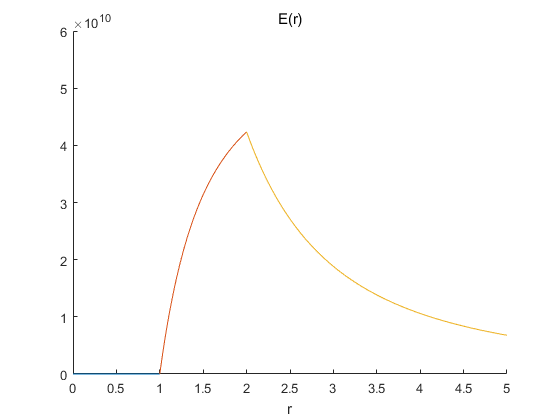
\includegraphics[width=7.0cm]{p2.png}}
  \centerline{$E(r)$}
\end{minipage}
\hfill
\begin{minipage}{.48\linewidth}
  \centerline{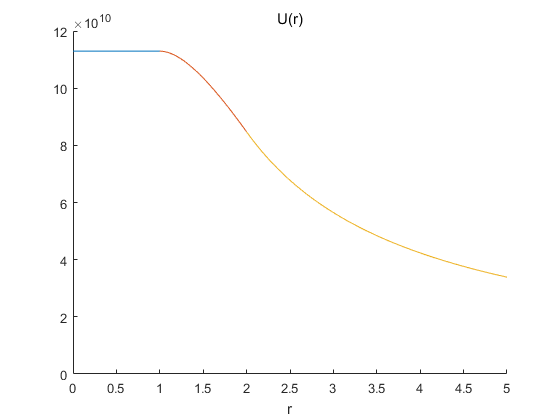
\includegraphics[width=7.0cm]{p2_2.png}}
  \centerline{$U(r)$}
\end{minipage}
\caption{$E(r)$ and $U(r)$}
\label{fig-5}
\end{figure}

When $r\geqslant b$,
$$U(r)=\int_r^{\infty}\frac{k(b^2-a^2)}{2\varepsilon_0r^2}dr=\frac{k}{2\varepsilon_0r}(b^2-a^2)$$
When $a\leqslant r<b$,
$$U(r)=\int_r^b\frac{k(r^2-a^2)}{2\varepsilon_0r^2}dr+U(b)=\frac{k}{2\varepsilon_0r}(2br-r^2-a^2)$$
When $r<a$,
$$U(r)=U(a)=\frac{k}{\varepsilon_0}(b-a)$$
\end{enumerate}

\section{}
$$E(r)\cdot2\pi rl=\frac{\lambda l}{\varepsilon_0}$$
$$E(r)=\frac{\lambda}{2\pi r\varepsilon_0}$$
Choose a point of distance R away from the wire as the reference point.
$$U=\int_s^R\frac{\lambda}{2\pi r\varepsilon_0}dr=\frac{\lambda}{2\pi\varepsilon_0}ln\frac{R}{s}$$
Suppose the wire to be x-axis and the line of distance from the wire and the point to be the y-axis.
$$\nabla U=-\frac{\lambda}{2\pi s\varepsilon_0}\hat{n_y}$$
$$\bar{E}=-\nabla U=\frac{\lambda}{2\pi s\varepsilon_0}\hat{n_y}$$
So it yields the correct field.

\section{}

\begin{align*}
U_A&=\int_0^h\frac{1}{4\pi\varepsilon_0}\cdot\frac{\sigma\cdot2\pi r\sqrt{2}dr}{\sqrt{2}r}=\frac{\sigma h}{2\varepsilon_0}\\
U_B&=\int_0^h\frac{1}{4\pi\varepsilon_0}\cdot\frac{\sigma\cdot2\pi r\sqrt{2}dr}{\sqrt{(h-r)^2+r^2}}\\
&=\frac{\sqrt{2}\sigma}{2\varepsilon_0}\left(\frac{1}{2}\sqrt{(h-r)^2+r^2}+\frac{h}{2\sqrt{2}}ln|4r-2h+2\sqrt{2}\sqrt{(h-r)^2+r^2}|\right)\bigg|_0^h\\
&=\frac{\sqrt{2}\sigma}{2\varepsilon_0}\left(\frac{h-h}{2}+\frac{h}{2\sqrt{2}}ln\left|\frac{2h+2\sqrt{2}h}{-2h+2\sqrt{2}h}\right|\right)\\
&=\frac{\sigma h}{2\varepsilon_0}ln(1+\sqrt{2})\\
\Delta U&=U_B-U_A=\frac{\sigma h}{2\varepsilon_0}[ln(1+\sqrt{2})-1]
\end{align*}

\section{}
\begin{align*}
q&=\int\rho dV=\int_0^r4\pi r^2\rho dr=\int_0^r-\frac{4\textbf{e}r^2}{a^3}e^{-\frac{2r}{a}}dr=\frac{e}{2}\int_0^{-\frac{2r}{a}}u^2e^udu\\
&=\frac{\textbf{e}}{2}(u^2-2u+2)e^u\bigg|_0^{-\frac{2r}{a}}=\frac{\textbf{e}}{2}\left[\left(\frac{4r^2}{a^2}+\frac{4r}{a}+2\right)e^{-\frac{2r}{a}}-2\right]\\
&=\textbf{e}\left[\left(\frac{2r^2}{a^2}+\frac{2r}{a}+1\right)e^{-\frac{2r}{a}}-1\right]
\end{align*}
$$E\cdot4\pi r^2=\frac{q}{\varepsilon_0}$$
$$\bar{E}=\frac{\textbf{e}}{4\pi\varepsilon_0}\left[\left(\frac{2}{a^2}+\frac{2}{ar}+\frac{1}{r^2}\right)e^{-\frac{2r}{a}}-\frac{1}{r^2}\right]\hat{n_r}$$
$$V=\int_r^{\infty}Edr=\frac{\textbf{e}}{4\pi\varepsilon_0}\left(-\frac{a+r}{ar}e^{-\frac{2r}{a}}+\frac{1}{r}\right)\bigg|_r^{\infty}
=\frac{\textbf{e}}{4\pi r\varepsilon_0}\left(\frac{a+r}{a}e^{-\frac{2r}{a}}-1\right)$$
When $r\to0$, $E\to-\infty$, $V\to-\infty$\\
When $r\to\infty$, $E\to0$, $V\to0$\\
They are similar to a point charge $-e$ placed at the origin.
\begin{figure}[h!]
	\centering
	\subfigure[$E(r)$]{
	\label{Fig.sub.1}
	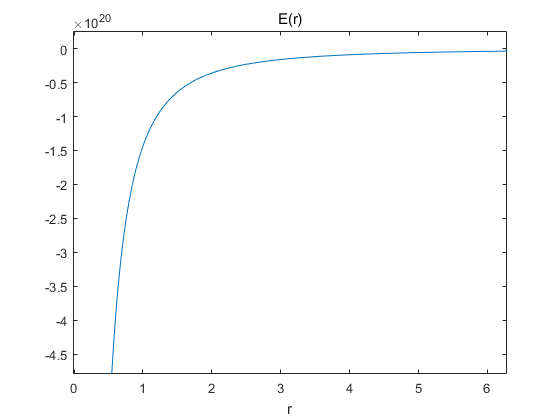
\includegraphics[width=7cm]{p5.png}}
	\subfigure[$V(r)$]{
	\label{Fig.sub.2}
	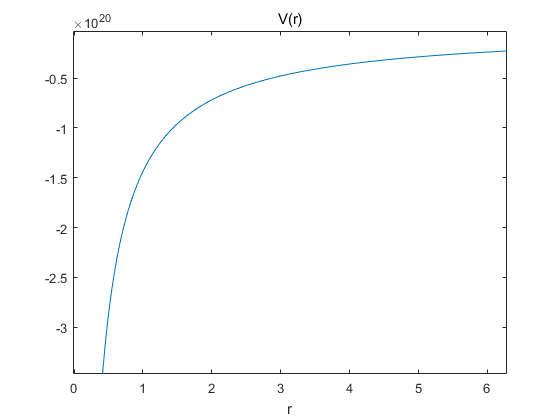
\includegraphics[width=7cm]{p5_2.png}}
	\caption{$E(r)$ and $V(r)$}
	\label{fig-5}
\end{figure}

\section{}
\begin{enumerate}[(a)]
\item
$$V=\int_r^R\frac{q}{4\pi r^2\varepsilon_0}\frac{r^3}{R^3}dr+\int_R^{\infty}\frac{q}{4\pi r^2\varepsilon_0}dr
=\frac{q}{4\pi\varepsilon_0}\left[\frac{\frac{1}{2}(R^2-r^2)}{R^3}+\frac{1}{R}\right]
=\frac{q}{8\pi R^3\varepsilon_0}(3R^2-r^2)$$
$$U_{conf}=\frac{1}{2}\int_{\Omega}\frac{q}{\frac{4}{3}\pi R^3}\frac{q}{8\pi R^3\varepsilon_0}(3R^2-r^2)d\tau=\frac{3q^2}{8\pi R^6\varepsilon_0}\int_0^Rr^2(3R^2-r^2)dr=\frac{3q^2}{20\pi R\varepsilon_0}$$
\item
\begin{align*}
U_{conf}&=\frac{\varepsilon_0}{2}\left(\int_{\Omega_1}E_1^2d\tau+\int_{\Omega_2}E_2^2d\tau\right)\\
&=\frac{\varepsilon_0}{2}\left[\int_0^R\left(\frac{q}{4\pi r^2\varepsilon_0}\frac{r^3}{R^3}\right)^24\pi r^2dr+\int_R^{\infty}\left(\frac{q}{4\pi r^2\varepsilon_0}\right)^24\pi r^2dr\right]\\
&=\frac{q^2}{8\pi\varepsilon_0}\left(\int_0^R\frac{r^4}{R^6}dr+\int_R^{\infty}\frac{1}{r^2}dr\right)\\
&=\frac{3q^2}{20\pi R\varepsilon_0}
\end{align*}
\item
\begin{align*}
U_{conf}&=\frac{\varepsilon_0}{2}\left(\int_{\Omega}E^2d\tau+\oint_{\Sigma}VEdA\right)\\
&=\frac{\varepsilon_0}{2}\left[\int_0^R\left(\frac{q}{4\pi r^2\varepsilon_0}\frac{r^3}{R^3}\right)^24\pi r^2dr+\int_R^{\infty}\frac{q}{4\pi r^2\varepsilon_0}dr\frac{q}{4\pi a^2\varepsilon_0}\cdot4\pi a^2\right]\\
&=\frac{q^2}{8\pi\varepsilon_0}\left(\int_0^R\frac{r^4}{R^6}dr+\int_R^{\infty}\frac{1}{r^2}dr\right)\\
&=\frac{3q^2}{20\pi R\varepsilon_0}
\end{align*}
When $a\to\infty$, $\oint_{\Sigma}VEdA\to0$, $U_{conf}=\frac{\varepsilon_0}{2}\int_{all\ space}E^2d\tau$
\item
$$Q=\frac{qr^3}{R^3}$$
$$dQ=\frac{3qr^2dr}{R^3}$$
$$\int\frac{Q}{4\pi r\varepsilon}dQ=\int_0^R\frac{3q^2r^4}{4\pi R^6\varepsilon_0}dr=\frac{3q^2}{20\pi R\varepsilon_0}$$

\end{enumerate}

\section{}
$$q=0$$
$$\nabla^2V=0$$
Since $V$ is specified on the boundary of $\Omega$, the solution to the equation is unique.\\
Only when $V$ is a constant, the solution is unique.\\
So the electric potential inside is constant, which means $E=0$ there.

\section{}
\begin{enumerate}[(a)]
\item
\begin{align*}
V&=\frac{q}{4\pi\varepsilon_0}\left[\frac{1}{\sqrt{x^2+y^2+(z-d)^2}}-\frac{1}{\sqrt{x^2+y^2+(z+d)^2}}\right]\\
\sigma&=-\varepsilon_0\frac{\partial V}{\partial z}\bigg|_{z=0}\\
&=-\frac{q}{4\pi}\lbrace(2z+d)[x^2+y^2+(z+d)^2]^{-\frac{3}{2}}-(2z-d)[x^2+y^2+(z-d)^2]^{-\frac{3}{2}}\rbrace\bigg|_{z=0}\\
&=-\frac{qd}{2\pi}(r^2+d^2)^{-\frac{3}{2}}
\end{align*}
\item
$$q_i=\int_0^{2\pi}\int_0^{\infty}\sigma rdrd\theta=-qd\int_0^{\infty}\frac{r}{(r^2+d^2)^{\frac{3}{2}}}dr=qd\frac{1}{\sqrt{r^2+d^2}}\bigg|_0^{\infty}=-q$$
\end{enumerate}

\section{}
Suppose the line from the center of the ball to the point charge to be the z-axis and the plane perpendicular to be the xy-plane.
$$r=\sqrt{x^2+y^2+(z-d)^2}$$
$$r'=\sqrt{x^2+y^2+(z-d')^2}$$
$$\frac{1}{4\pi\varepsilon_0}\left(\frac{q}{r}+\frac{q'}{r'}\right)=0$$
\begin{equation*}
\left\lbrace
\begin{array}{cc}
(R^2+d^2)q'^2-(R^2+d'^2)q^2&=0\\
2R(dq'^2-d'q^2)&=0
\end{array}
\right.\Rightarrow\left\lbrace
\begin{array}{cc}
q'&=-\frac{R}{d}q\\
d'&=\frac{R^2}{d}
\end{array}
\right.
\end{equation*}
$$V(x,y,z)=\frac{q}{4\pi\varepsilon_0}\left[\frac{1}{\sqrt{x^2+y^2+(z-d)^2}}-\frac{R}{d\sqrt{x^2+y^2+(z+\frac{R^2}{d})^2}}\right]$$

\section{}
Suppose the line from the center of the ball to the point charge to be the z-axis and the plane perpendicular to be the xy-plane.\\
According to Problem 9,
\begin{equation*}
\left\lbrace
\begin{array}{cc}
q'&=-\frac{R}{d}q\\
d'&=\frac{R^2}{d}
\end{array}
\right.
\end{equation*}
Since the ball in ungrounded, we need another $q''$ to cancel out electric potential on the ball.
$$q''=-Q-q'=-Q+\frac{R}{d}q$$
$$r''=\sqrt{x^2+y^2+z^2}$$
\begin{align*}
V(x,y,z)&=\frac{1}{4\pi\varepsilon_0}\left(\frac{q}{r}+\frac{q'}{r'}+\frac{q''}{r''}\right)\\
&=\frac{1}{4\pi\varepsilon_0}\left[\frac{q}{\sqrt{x^2+y^2+(z-d)^2}}-\frac{qR}{d\sqrt{x^2+y^2+(z+\frac{R^2}{d})^2}}+\frac{-Q+\frac{R}{d}q}{\sqrt{x^2+y^2+z^2}}\right]
\end{align*}

\section{}
\begin{enumerate}[(a)]
\item
We need three charges.\\
One point charge $q$ at $(-b,-a)$\\
Two point charge $-q$ at $(-b,a)$ and $(b,-a)$
\item
\begin{align*}
F&=\frac{q^2}{4\pi\varepsilon_0}\left(-\frac{1}{4b^2}\hat{n_x}-\frac{1}{4a^2}\hat{n_y}+\frac{1}{4a^2+4b^2}\frac{b\hat{n_x}+a\hat{n_y}}{\sqrt{a^2+b^2}}\right)\\
&=\frac{q^2}{4\pi\varepsilon_0}\left[\left(\frac{b}{4(a^2+b^2)^{\frac{3}{2}}}-\frac{1}{4b^2}\right)\hat{n_x}+\left(\frac{a}{4(a^2+b^2)^{\frac{3}{2}}}-\frac{1}{4a^2}\right)\hat{n_y}\right]
\end{align*}
\item
$$V=\frac{q}{4\pi\varepsilon_0}\left(\frac{1}{2\sqrt{a^2+b^2}}-\frac{1}{2a}-\frac{1}{2b}\right)$$
$$W=\frac{q^2}{8\pi\varepsilon_0}\left(\frac{1}{\sqrt{a^2+b^2}}-\frac{1}{a}-\frac{1}{b}\right)$$
\item
No, the method works only when the angle $\theta=\frac{\pi}{k},k\geq2,k\in Z$\\
It is because the point charge should be imaged $k+2$ times and then the next image is the charge itself. If $k$ is not a normal number, it doesn't work.
\end{enumerate}


\end{document}
